\documentclass[12pt]{article}

\usepackage{graphicx}

\title{PEM Numerical Analysis}
\author{B. Giffin}
\date{\today}

\begin{document}
%\maketitle

\section*{In Pursuit of An Alternative Formulation for Quadratically Complete PEM Elements}

Herein we discuss an alternative formulation for quadratically complete PEM elements.

\subsection*{The Original Approach}

Consider a representative 1D PEM element $\Omega$ subdivided into a number of segments $\gamma_b$ and verticies $v_a$. Let us further suppose that at least three of the verticies are classified as nodes $N_A$, whose shape function values $\varphi_N$ are known. We seek a linear transformation $\mathbf{M} : u_N \mapsto u|_{\gamma_b}$ such that the mapping $\mathbf{M}$ yields a piece-wise representation of $u|_{\gamma_b}$ on the set of segments which is both relatively ``smooth'' and ``continuous.'' More precisely, we require that any $u|_{\gamma_b}$ obtained through $\mathbf{M}$ be the unique minimizer of a prescribed functional $\mathcal{F}$:
\begin{equation}
        \mathcal{F} := \beta_0 \sum_{a \in \bar{\mathcal{B}}} \frac{h_a}{2} [\![ u ]\!]^2 \bigg|_{v_a} + \beta_1 \sum_{a \in \mathcal{B}} \frac{h_a^3}{2} [\![ n \nabla u ]\!]^2 \bigg|_{v_a}
\end{equation}
which represents a weighted measure of compatibility and smoothness in the piece-wise representation of $u$ over the element's segment partition. We will choose to represent each $u|_{\gamma_b}$ using a monomial basis, i.e.
\begin{equation}
     u |_{\gamma_b} (x) = \sum_{\alpha \leq k} a_{\gamma_b}^{(\alpha)} x^{\alpha} = \mathbf{m} \cdot \mathbf{a}_{\gamma_b}
\end{equation}
where $\mathbf{m}$ is a vector of monomials and $\mathbf{a}_{\gamma_b}$ is a vector of the corresponding (unknown) monomial coefficients for a given segment $\gamma_b$. Now, denote $\mathbf{a}$ as the vector of all segment monomial coefficients, and denote $\mathbf{u}$ as the vector of all nodal values. We may then formulate our minimum problem as
\begin{equation}
        \min_{\mathbf{a}} \mathcal{F} (\mathbf{a}, \mathbf{u}),
\end{equation}
and the unique minimizer of $\mathcal{F}$ will satisfy
\begin{equation}
        \frac{\partial \mathcal{F}}{\partial \mathbf{a}} = \mathbf{0}.
\end{equation}

Let us momentarily consider an individual vertex $v_a$ which separates two segments, $\gamma_{a1}$ and $\gamma_{a2}$. Note that
\begin{equation}
        h_a [\![ u ]\!]^2 \bigg|_{v_a} = (\mathbf{a}_{\gamma_{a1}} - \mathbf{a}_{\gamma_{a2}}) \cdot \left[ h_a \mathbf{m}_{v_a} \otimes \mathbf{m}_{v_a} \right] (\mathbf{a}_{\gamma_{a1}} - \mathbf{a}_{\gamma_{a2}}),
\end{equation}
and
\begin{equation}
        h_a^3 [\![ n \nabla u ]\!]^2 \bigg|_{v_a} = (\mathbf{a}_{\gamma_{a1}} - \mathbf{a}_{\gamma_{a2}}) \cdot \left[ h_a^3 \frac{\partial \mathbf{m}_{v_a}}{\partial n} \otimes \frac{\partial \mathbf{m}_{v_a}}{\partial n} \right] (\mathbf{a}_{\gamma_{a1}} - \mathbf{a}_{\gamma_{a2}}),
\end{equation}
where we prescribe $h_a = (|\gamma_{a1}| + |\gamma_{a2}|)$ to obtain a proportional scaling of the two integral contributions to $\mathcal{F}$. If we define moment matrices $\mathbf{J}_{0a}$ and $\mathbf{J}_{1a}$ as
\begin{equation}
        \mathbf{J}_{0a} \equiv h_a \mathbf{m}_{v_a} \otimes \mathbf{m}_{v_a}
\end{equation}
\begin{equation}
        \mathbf{J}_{1a} \equiv h_a^3 \frac{\partial \mathbf{m}_{v_a}}{\partial n} \otimes \frac{\partial \mathbf{m}_{v_a}}{\partial n}
\end{equation}
then we may express the local contribution from vertex $v_a$ to $\mathcal{F}$ as
\begin{equation}
        \mathcal{F}_a = \frac{1}{2} \left\{ \begin{array}{c} \mathbf{a}_{\gamma_{a1}} \\ \mathbf{a}_{\gamma_{a2}} \end{array} \right\} \cdot \bigg( \beta_0 \left[ \begin{array}{cc} \mathbf{J}_{0a} & - \mathbf{J}_{0a} \\ - \mathbf{J}_{0a} & \mathbf{J}_{0a} \end{array} \right] + \beta_1 \left[ \begin{array}{cc} \mathbf{J}_{1a} & - \mathbf{J}_{1a} \\ - \mathbf{J}_{1a} & \mathbf{J}_{1a} \end{array} \right] \bigg) \left\{ \begin{array}{c} \mathbf{a}_{\gamma_{a1}} \\ \mathbf{a}_{\gamma_{a2}} \end{array} \right\},
\end{equation}
or more concisely:
\begin{equation}
        \mathcal{F}_a = \frac{1}{2} \mathbf{a}_{\gamma_{a_{1,2}}} \cdot \mathbf{J}_a \mathbf{a}_{\gamma_{a_{1,2}}}.
\end{equation}
The matrix $\mathbf{J}_a$ expressed in the above equation constitutes a local contribution from vertex $v_a$ to the Jacobian of $\partial \mathcal{F} / \partial \mathbf{a}$ (i.e. to $\mathbf{J} = \partial^2 \mathcal{F} / \partial \mathbf{a} \, \partial \mathbf{a}$, which will ultimately be inverted when we solve for the unknown monomial coefficients in each segment).

If the particular vertex in question had been a node, then
\begin{equation}
        \mathcal{F}_a = \beta_0 \frac{h_a}{2} [\![ u ]\!]^2 \bigg|_{v_a} = \sum_i \left[ \frac{1}{2} \mathbf{a}_{\gamma_{a_{i}}} \cdot \mathbf{J}_{0a} \mathbf{a}_{\gamma_{a_{i}}} - \mathbf{a}_{\gamma_{a_{i}}} \cdot \mathbf{B}_{0a} u_a + \frac{1}{2} u_a A_{0a} u_a \right]
\end{equation}
where $u_a$ denotes the nodal value at vertex $v_a$, $h_a = \sum_i |\gamma_{a_i}|$, and
\begin{equation}
	A_{0a} \equiv \beta_0 h_a, \qquad \mathbf{B}_{0a} \equiv \beta_0 h_a \mathbf{m}_{v_a}.
\end{equation}
If we sum the contributions from all verticies, then we are justified in writing $\mathcal{F}$ as a quadratic form:
\begin{equation}
        \mathcal{F} (\mathbf{a}, \mathbf{u}) = \frac{1}{2} \mathbf{a} \cdot \mathbf{J} \mathbf{a} - \mathbf{a} \cdot \mathbf{B} \mathbf{u} + \frac{1}{2} \mathbf{u} \cdot \mathbf{A} \mathbf{u}.
\end{equation}

\subsection*{The Proposed Alternative Approach}

Let us propose the following representation for the element's shape functions defined on the set of all segments $\gamma_b$: suppose there exists some quadratic polynomial function $q(x) = \mathbf{m} \cdot \mathbf{a}_q$ such that $u |_{\gamma_b} = q + \hat{u} |_{\gamma_b}$, where the local segment functions $\hat{u} |_{\gamma_b} = \mathbf{m} \cdot \hat{\mathbf{a}}_{\gamma_b}$ are at most linear polynomials obtained from the solution of
\begin{equation}
	\min_{\hat{\mathbf{a}}, \mathbf{a}_q} \mathcal{F} (\hat{\mathbf{a}}, \hat{\mathbf{u}})
\end{equation}
with
\begin{equation}
	\hat{u}_a = u_a - \mathbf{m}_{v_a} \cdot \mathbf{a}_q,
\end{equation}
or in matrix form
\begin{equation}
	\hat{\mathbf{u}} = \mathbf{u} - \mathbf{Q} \mathbf{a}_q.
\end{equation}
Thus, we must solve the augmented minimum problem
\begin{equation}
	\min_{\hat{\mathbf{a}}, \mathbf{a}_q} \mathcal{F} (\hat{\mathbf{a}}, \mathbf{u} - \mathbf{Q} \mathbf{a}_q)
\end{equation}
for both $\mathbf{a}_q$ (the element-wide quadratic coefficients), and $\hat{\mathbf{a}}$ (the ``residual'' segment coefficients) for a given setting of nodal values $\mathbf{u}$. Explicitly:
\begin{equation}
        \mathcal{F} (\hat{\mathbf{a}}, \mathbf{u} - \mathbf{Q} \mathbf{a}_q) = \frac{1}{2} \hat{\mathbf{a}} \cdot \mathbf{J} \hat{\mathbf{a}} - \hat{\mathbf{a}} \cdot \mathbf{B} (\mathbf{u} - \mathbf{Q} \mathbf{a}_q) + \frac{1}{2} (\mathbf{u} - \mathbf{Q} \mathbf{a}_q) \cdot \mathbf{A} (\mathbf{u} - \mathbf{Q} \mathbf{a}_q),
\end{equation}
and
\begin{equation}
	\frac{\partial \mathcal{F}}{\partial \hat{\mathbf{a}}} = \mathbf{J} \hat{\mathbf{a}} - \mathbf{B} (\mathbf{u} - \mathbf{Q} \mathbf{a}_q) = \mathbf{0},
\end{equation}
\begin{equation}
	\frac{\partial \mathcal{F}}{\partial \mathbf{a}_q} = \hat{\mathbf{a}} \cdot \mathbf{B} \mathbf{Q} - \mathbf{Q}^T \mathbf{A} (\mathbf{u} - \mathbf{Q} \mathbf{a}_q) = \mathbf{0},
\end{equation}
\begin{equation}
	\left[ \begin{array}{cc} \mathbf{J} & \mathbf{B} \mathbf{Q} \\ \mathbf{Q}^T \mathbf{B}^T & \mathbf{Q}^T \mathbf{A} \mathbf{Q} \end{array} \right] \left\{ \begin{array}{c} \hat{\mathbf{a}} \\ \mathbf{a}_q \end{array} \right\} = \left[ \begin{array}{c} \mathbf{B} \\ \mathbf{Q}^T \mathbf{A} \end{array} \right] \left\{ \begin{array}{c} \mathbf{u} \end{array} \right\},
\end{equation}
or more succinctly,
\begin{equation}
	\mathbf{M}_a \mathbf{a} = \mathbf{M}_u \mathbf{u}
	\label{eq:final}
\end{equation}
where $\mathbf{a}$ now denotes the vector of all unknown polynomial coefficients (both $\hat{\mathbf{a}}$ and $\mathbf{a}_q$).

\newpage

\subsection*{Preliminary Results}

A simple MATLAB test script was created for the 1D PEM problem depicted in Figure \ref{fig:1dpem}.
\begin{figure}[!h]
  \centering
  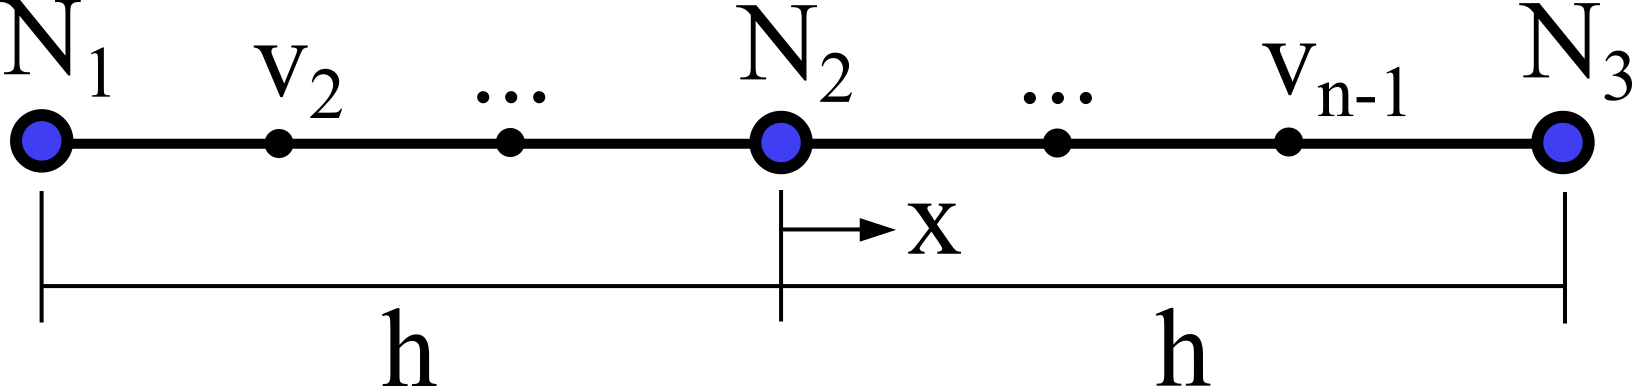
\includegraphics[width=0.7\textwidth]{1dpem.png}
  \caption{A representative 1D partitioned element, $\Omega$.}
  \label{fig:1dpem}
\end{figure}
This test was constructed to verify the completeness of the resulting shape functions, and to determine the rank sufficiency (or the condition number) of the system of equations expressed in (\ref{eq:final}).

\begin{figure}[!ht]
  \centering
  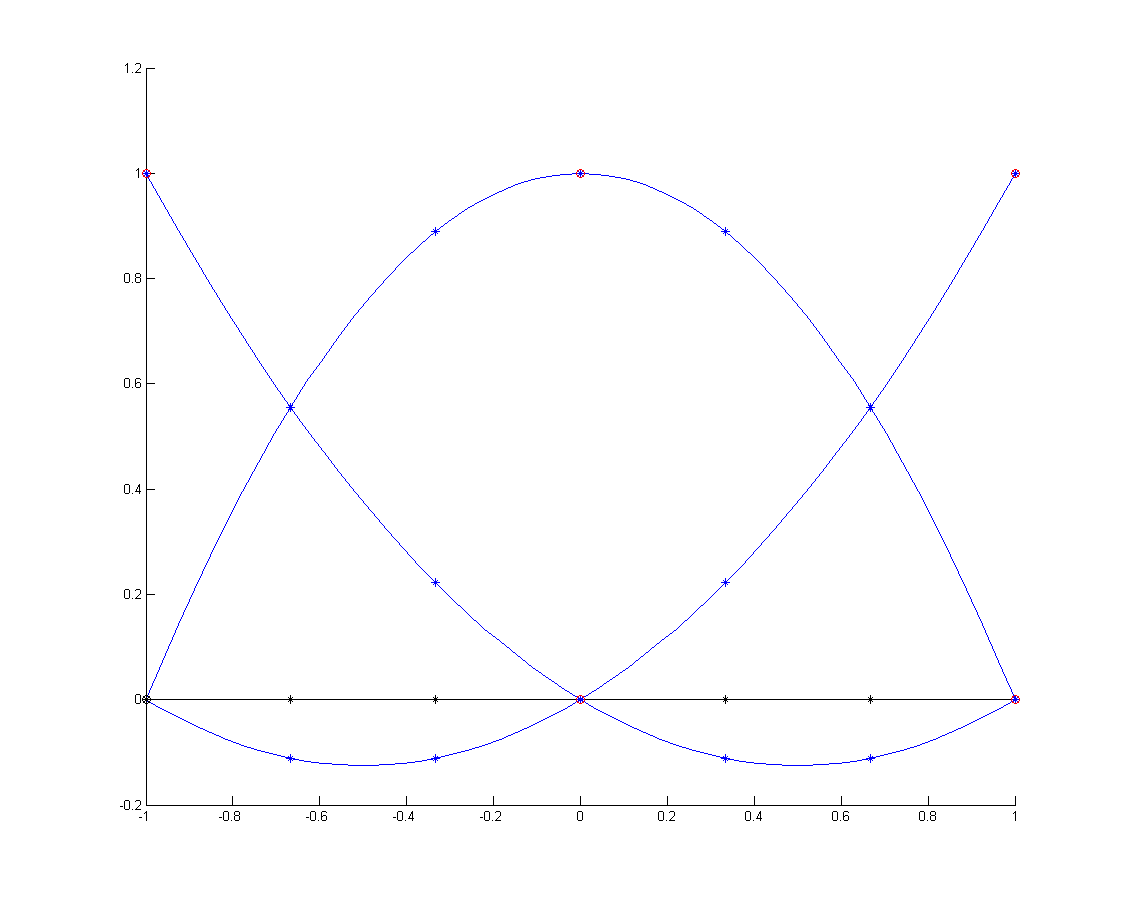
\includegraphics[width=0.9\textwidth]{lagrange.png}
  \caption{The resulting PEM quadratic nodal interpolants (consistent with the Lagrange interpolating polynomials).}
  \label{fig:lagrange}
\end{figure}

Initial attempts pursued the case where $q(x)$ was allowed to be an arbitrary quadratic function (i.e. $q(x) = a_q^{(0)} + a_q^{(1)} x + a_q^{(2)} x^2$), and where each segment's local variations $\hat{u} |_{\gamma_b}$ were prescribed to be arbitrary linear functions (i.e. $\hat{u} |_{\gamma_b} = \hat{a}_{\gamma_b}^{(0)} + \hat{a}_{\gamma_b}^{(1)} x$), such that the resulting shape functions in a given segment assumed the form:
\begin{equation}
	u |_{\gamma_b} = (a_q^{(0)} + \hat{a}_{\gamma_b}^{(0)}) + (a_q^{(1)} + \hat{a}_{\gamma_b}^{(1)}) x + a_q^{(2)} x^2.
\end{equation}
This, however, led $\mathbf{M}_a$ to be rank deficient, as the constant and linear coefficients could take on arbitrary non-zero values such that $a_q^{(0)} = - \hat{a}_{\gamma_b}^{(0)}$ or $a_q^{(1)} = - \hat{a}_{\gamma_b}^{(1)}$, even if the nodal values were identically zero. Consequently, it was observed that any enrichment $q(x)$ would need to consist of polynomials not already contained in the space of piece-wise linear polynomials represented by the segment coefficients. 


Secondary attempts which restricted $q(x)$ to be a second-order monomial (i.e. $q(x) = a_q^{(2)} x^2$) succeeded in achieving rank-sufficiency, and produced shape functions which were quadratically complete (see Figure \ref{fig:lagrange}.)


An examination of the condition number for $\mathbf{M}_a$ via a parameter sensitivity analysis revealed that $\kappa (\mathbf{M}_a) \approx O (h^4)$ (consistent with the $O (h^{2k})$ approximation, derived previously), in affirmation of previous speculation that ill-conditioning in the PEM linear systems is largely a consequence of the choice of polynomial basis (namely, the monomial basis).

\newpage

\subsection*{The Revised Alternative Approach}

Once again, we propose the following representation for the element's shape functions defined on the set of all segments $\gamma_b$: suppose there exists some quadratic polynomial function $q(x) = \mathbf{m} \cdot \mathbf{a}_q$ such that $u |_{\gamma_b} = q + \hat{u} |_{\gamma_b}$, where the local segment functions $\hat{u} |_{\gamma_b} = \mathbf{m} \cdot \hat{\mathbf{a}}_{\gamma_b}$ are at most linear polynomials obtained from the solution of
\begin{equation}
	\min_{\hat{\mathbf{a}}} \mathcal{F} (\hat{\mathbf{a}}, \hat{\mathbf{u}})
\end{equation}
with
\begin{equation}
	\hat{u}_a = u_a - \mathbf{m}_{v_a} \cdot \mathbf{a}_q,
\end{equation}
or in matrix form
\begin{equation}
	\hat{\mathbf{u}} = \mathbf{u} - \mathbf{Q} \mathbf{a}_q.
\end{equation}
We will proceed by first solving the augmented minimum problem for $\hat{\mathbf{a}}$ only, holding the residual nodal values $\hat{\mathbf{u}}$ fixed. Explicitly:
\begin{equation}
        \mathcal{F} (\hat{\mathbf{a}}, \hat{\mathbf{u}}) = \frac{1}{2} \hat{\mathbf{a}} \cdot \mathbf{J} \hat{\mathbf{a}} - \hat{\mathbf{a}} \cdot \mathbf{B} \hat{\mathbf{u}} + \frac{1}{2} \hat{\mathbf{u}} \cdot \mathbf{A} \hat{\mathbf{u}},
\end{equation}
and
\begin{equation}
	\frac{\partial \mathcal{F}}{\partial \hat{\mathbf{a}}} = \mathbf{J} \hat{\mathbf{a}} - \mathbf{B} \hat{\mathbf{u}} = \mathbf{0},
\end{equation}
such that we may write $\hat{\mathbf{a}}$ directly in terms of $\hat{\mathbf{u}}$:
\begin{equation}
	\hat{\mathbf{a}} = \mathbf{J}^{-1} \mathbf{B} \hat{\mathbf{u}}.
\end{equation}
Substituting this expression back into $\mathcal{F}$, we obtain
\begin{equation}
        \mathcal{F} (\hat{\mathbf{u}}) = \frac{1}{2} (\mathbf{J}^{-1} \mathbf{B} \hat{\mathbf{u}}) \cdot \mathbf{J} (\mathbf{J}^{-1} \mathbf{B} \hat{\mathbf{u}}) - (\mathbf{J}^{-1} \mathbf{B} \hat{\mathbf{u}}) \cdot \mathbf{B} \hat{\mathbf{u}} + \frac{1}{2} \hat{\mathbf{u}} \cdot \mathbf{A} \hat{\mathbf{u}},
\end{equation}
\begin{equation}
        \mathcal{F} (\hat{\mathbf{u}}) = \frac{1}{2} \hat{\mathbf{u}} \cdot (\mathbf{A} - \mathbf{B}^T \mathbf{J}^{-1} \mathbf{B}) \hat{\mathbf{u}} = \frac{1}{2} \hat{\mathbf{u}} \cdot \mathbf{D} \hat{\mathbf{u}}
\end{equation}
or
\begin{equation}
        \mathcal{F} (\mathbf{a}_q, \mathbf{u}) = \frac{1}{2} \mathbf{u} \cdot \mathbf{D} \mathbf{u} - \mathbf{u} \cdot \mathbf{D} \mathbf{Q} \mathbf{a}_q + \frac{1}{2} \mathbf{a}_q \cdot \mathbf{Q}^T \mathbf{D} \mathbf{Q} \mathbf{a}_q.
\end{equation}
Now, minimizing this $\mathcal{F}$ with respect to $\mathbf{a}_q$, we arrive at
\begin{equation}
	\frac{\partial \mathcal{F}}{\partial \mathbf{a}_q} = \mathbf{Q}^T \mathbf{D} \mathbf{Q} \mathbf{a}_q - \mathbf{Q}^T \mathbf{D} \mathbf{u} = \mathbf{0},
\end{equation}
such that we may write $\mathbf{a}_q$ directly in terms of $\mathbf{u}$:
\begin{equation}
	\mathbf{a}_q = (\mathbf{Q}^T \mathbf{D} \mathbf{Q})^{-1} \mathbf{Q}^T \mathbf{D} \mathbf{u} = \bar{\mathbf{M}} \mathbf{u},
	\label{eq:aq}
\end{equation}
and because
\begin{equation}
	\hat{\mathbf{u}} = \mathbf{u} - \mathbf{Q} \mathbf{a}_q = (\mathbf{1} - \mathbf{Q} \bar{\mathbf{M}}) \mathbf{u},
\end{equation}
we may write $\hat{\mathbf{a}}$ directly in terms of $\mathbf{u}$, as well:
\begin{equation}
	\hat{\mathbf{a}} = \mathbf{J}^{-1} \mathbf{B} \hat{\mathbf{u}} = \mathbf{J}^{-1} \mathbf{B} (\mathbf{1} - \mathbf{Q} \bar{\mathbf{M}}) \mathbf{u} = \hat{\mathbf{M}} \mathbf{u}.
\end{equation}

The issue that arises with the aforementioned approach is that $\mathbf{D}$ (and $\mathbf{Q}^T \mathbf{D} \mathbf{Q}$, by extension) is only positive semi-definite, and therefore is not necessarily invertible. This is more intuitively understood if one considers the fact that $\mathcal{F}$ will attain its absolute minimum value (i.e. $0$) whenever the nodes are set consistent with any affine function, because the quasi-linear PEM function space is able to exactly reproduce such a function from the nodal data, such that all kinks and jumps are non-existent.

It may be insightful to briefly remark that the element-wide quadratic polynomial coefficients $\mathbf{a}_q$ are obtained in (\ref{eq:aq}) as a solution to the weighted least squares problem, i.e.
\begin{equation}
	\mathbf{a}_q = (\mathbf{X}^T \mathbf{W} \mathbf{X})^{-1} \mathbf{X}^T \mathbf{W} \mathbf{y}
\end{equation}
where $\mathbf{X} = \mathbf{Q}$, $\mathbf{W} = \mathbf{D}$, and $\mathbf{y} = \mathbf{u}$. The problem with the present formulation, however, is that $\mathbf{W}$ ($\mathbf{D}$ in our case) in not necessarily positive-definite, leading to a potential rank deficiency in the weighted least squares problem of interest. This can be remedied by a modification to $\mathcal{F} (\hat{\mathbf{a}}, \hat{\mathbf{u}})$ of the form:
\begin{equation}
        \mathcal{F} (\hat{\mathbf{a}}, \hat{\mathbf{u}}) = \frac{1}{2} \hat{\mathbf{a}} \cdot \mathbf{J} \hat{\mathbf{a}} - \hat{\mathbf{a}} \cdot \mathbf{B} \hat{\mathbf{u}} + \frac{1}{2} \hat{\mathbf{u}} \cdot (\mathbf{A} + \tilde{\mathbf{W}}) \hat{\mathbf{u}},
\end{equation}
where $\tilde{\mathbf{W}}$ effectively serves as a penalization of $\hat{\mathbf{u}}$ -- the residual nodal values. Intuitively, this modification seeks to minimize the residual nodal values which enter into the PEM functional, thereby allowing the element-wide enhancement terms to represent the constant and linear portions of the shape functions. Notably, this adjustment does not impact the computation of the residual shape functions. The only remaining question regards how to prescribe an appropriate penalization; one simple choice is $\tilde{\mathbf{W}} = \mathbf{A}$, consistent with the edge-functionals' proportional weighting of the nodes.

A further remark regarding the appropriateness of a quadratic enhancement to the internal displacement field of the element comes from the consideration of the F-test for the convergence of a non-conforming element formulation. If we permit the internal displacement field to vary according to an arbitrary quadratic determined from the nodal values alone, we run the risk of violating compatibility at inter-element interfaces, to such an extent that the element may fail the F-test. In these cases, it may be necessary to enforce the conditions of the strong F-test on every face of the element:
\begin{equation}
	\int_{F} \left[ u \right] \, da = 0 \quad \forall F,
\end{equation}
however, this may over-constrain the shape functions, such that higher-order completeness may be compromised.

A crazy idea comes from the virtual element method, which considers the $L^2$ projection of a function defined on the interior of the element onto a portion of the element's boundary. This projection could be effected rather simply by considering the restriction of 

\end{document}
